\documentclass[1p]{elsarticle_modified}
%\bibliographystyle{elsarticle-num}

%\usepackage[colorlinks]{hyperref}
%\usepackage{abbrmath_seonhwa} %\Abb, \Ascr, \Acal ,\Abf, \Afrak
\usepackage{amsfonts}
\usepackage{amssymb}
\usepackage{amsmath}
\usepackage{amsthm}
\usepackage{scalefnt}
\usepackage{amsbsy}
\usepackage{kotex}
\usepackage{caption}
\usepackage{subfig}
\usepackage{color}
\usepackage{graphicx}
\usepackage{xcolor} %% white, black, red, green, blue, cyan, magenta, yellow
\usepackage{float}
\usepackage{setspace}
\usepackage{hyperref}

\usepackage{tikz}
\usetikzlibrary{arrows}

\usepackage{multirow}
\usepackage{array} % fixed length table
\usepackage{hhline}

%%%%%%%%%%%%%%%%%%%%%
\makeatletter
\renewcommand*\env@matrix[1][\arraystretch]{%
	\edef\arraystretch{#1}%
	\hskip -\arraycolsep
	\let\@ifnextchar\new@ifnextchar
	\array{*\c@MaxMatrixCols c}}
\makeatother %https://tex.stackexchange.com/questions/14071/how-can-i-increase-the-line-spacing-in-a-matrix
%%%%%%%%%%%%%%%

\usepackage[normalem]{ulem}

\newcommand{\msout}[1]{\ifmmode\text{\sout{\ensuremath{#1}}}\else\sout{#1}\fi}
%SOURCE: \msout is \stkout macro in https://tex.stackexchange.com/questions/20609/strikeout-in-math-mode

\newcommand{\cancel}[1]{
	\ifmmode
	{\color{red}\msout{#1}}
	\else
	{\color{red}\sout{#1}}
	\fi
}

\newcommand{\add}[1]{
	{\color{blue}\uwave{#1}}
}

\newcommand{\replace}[2]{
	\ifmmode
	{\color{red}\msout{#1}}{\color{blue}\uwave{#2}}
	\else
	{\color{red}\sout{#1}}{\color{blue}\uwave{#2}}
	\fi
}

\newcommand{\Sol}{\mathcal{S}} %segment
\newcommand{\D}{D} %diagram
\newcommand{\A}{\mathcal{A}} %arc


%%%%%%%%%%%%%%%%%%%%%%%%%%%%%5 test

\def\sl{\operatorname{\textup{SL}}(2,\Cbb)}
\def\psl{\operatorname{\textup{PSL}}(2,\Cbb)}
\def\quan{\mkern 1mu \triangleright \mkern 1mu}

\theoremstyle{definition}
\newtheorem{thm}{Theorem}[section]
\newtheorem{prop}[thm]{Proposition}
\newtheorem{lem}[thm]{Lemma}
\newtheorem{ques}[thm]{Question}
\newtheorem{cor}[thm]{Corollary}
\newtheorem{defn}[thm]{Definition}
\newtheorem{exam}[thm]{Example}
\newtheorem{rmk}[thm]{Remark}
\newtheorem{alg}[thm]{Algorithm}

\newcommand{\I}{\sqrt{-1}}
\begin{document}

%\begin{frontmatter}
%
%\title{Boundary parabolic representations of knots up to 8 crossings}
%
%%% Group authors per affiliation:
%\author{Yunhi Cho} 
%\address{Department of Mathematics, University of Seoul, Seoul, Korea}
%\ead{yhcho@uos.ac.kr}
%
%
%\author{Seonhwa Kim} %\fnref{s_kim}}
%\address{Center for Geometry and Physics, Institute for Basic Science, Pohang, 37673, Korea}
%\ead{ryeona17@ibs.re.kr}
%
%\author{Hyuk Kim}
%\address{Department of Mathematical Sciences, Seoul National University, Seoul 08826, Korea}
%\ead{hyukkim@snu.ac.kr}
%
%\author{Seokbeom Yoon}
%\address{Department of Mathematical Sciences, Seoul National University, Seoul, 08826,  Korea}
%\ead{sbyoon15@snu.ac.kr}
%
%\begin{abstract}
%We find all boundary parabolic representation of knots up to 8 crossings.
%
%\end{abstract}
%\begin{keyword}
%    \MSC[2010] 57M25 
%\end{keyword}
%
%\end{frontmatter}

%\linenumbers
%\tableofcontents
%
\newcommand\colored[1]{\textcolor{white}{\rule[-0.35ex]{0.8em}{1.4ex}}\kern-0.8em\color{red} #1}%
%\newcommand\colored[1]{\textcolor{white}{ #1}\kern-2.17ex	\textcolor{white}{ #1}\kern-1.81ex	\textcolor{white}{ #1}\kern-2.15ex\color{red}#1	}

{\Large $\underline{11a_{291}~(K11a_{291})}$}

\setlength{\tabcolsep}{10pt}
\renewcommand{\arraystretch}{1.6}
\vspace{1cm}\begin{tabular}{m{100pt}>{\centering\arraybackslash}m{274pt}}
\multirow{5}{120pt}{
	\centering
	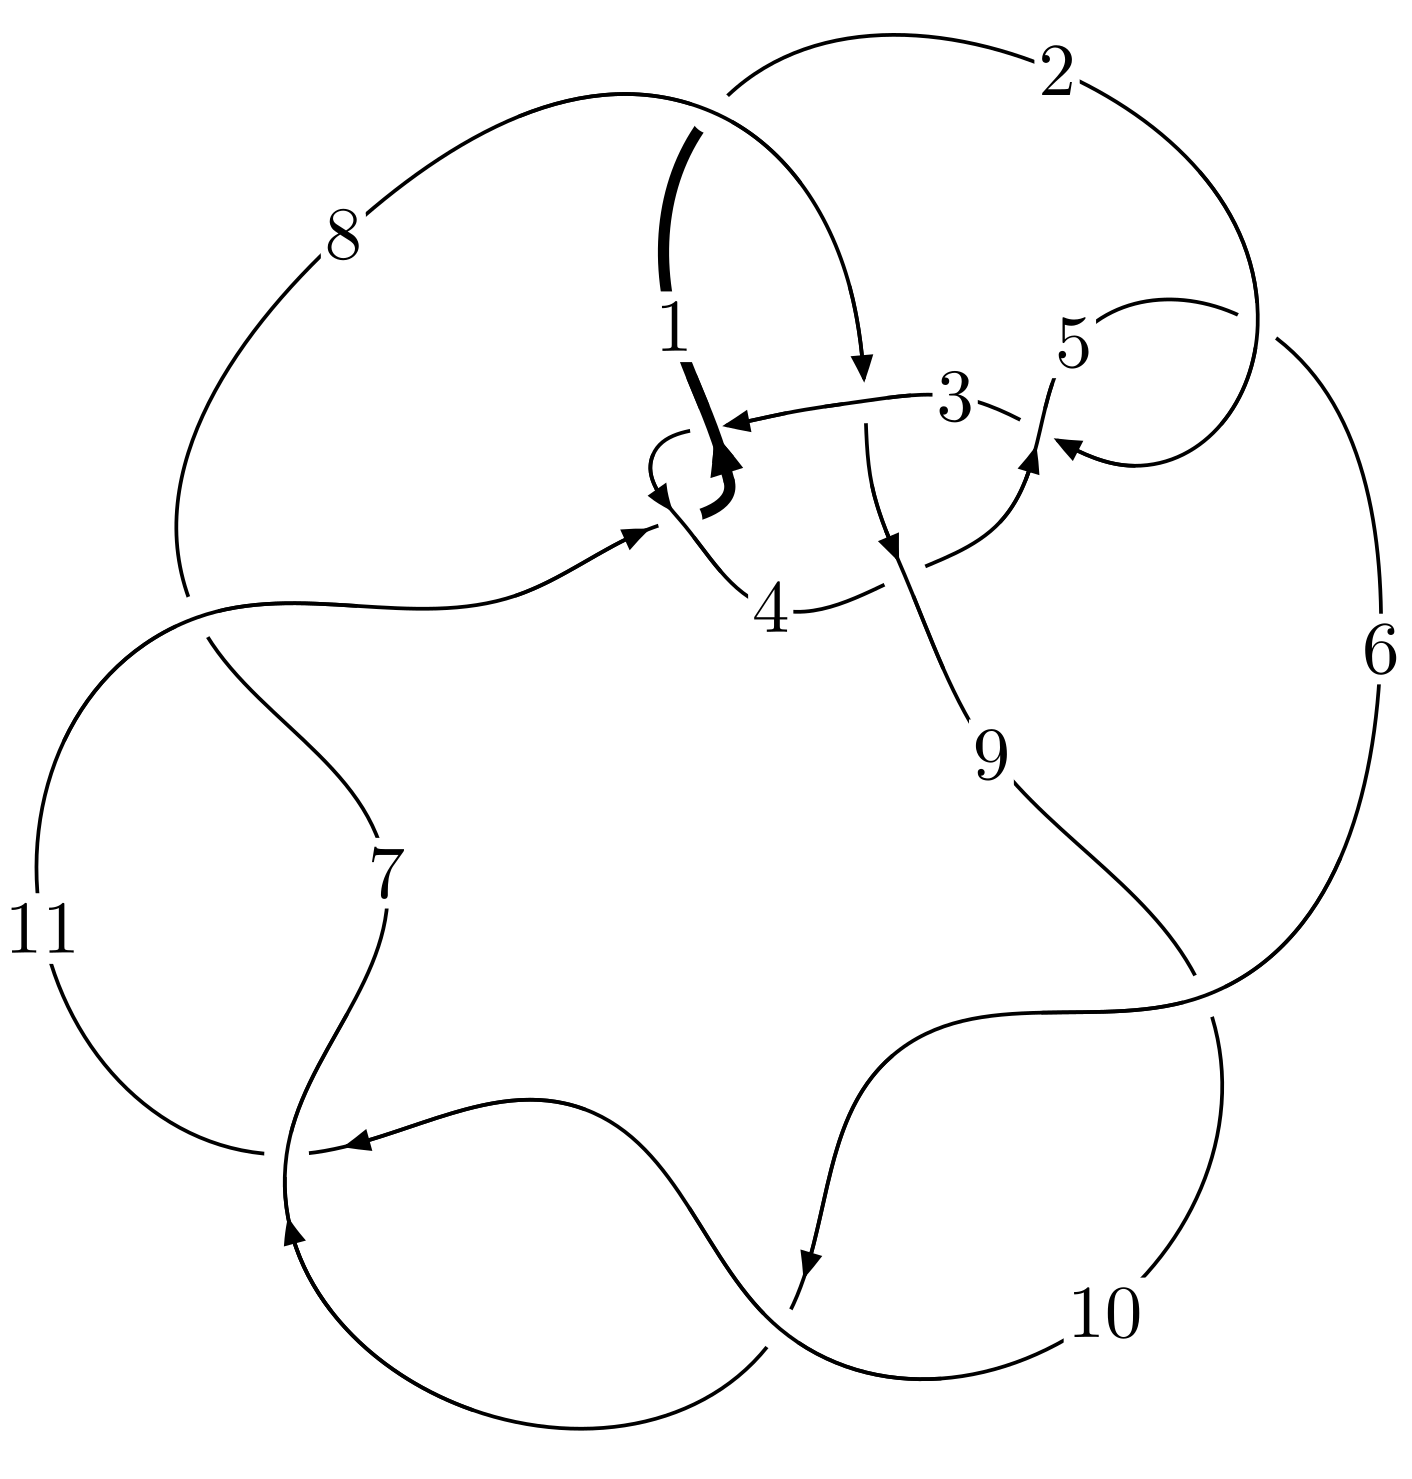
\includegraphics[width=112pt]{../../../GIT/diagram.site/Diagrams/png/540_11a_291.png}\\
\ \ \ A knot diagram\footnotemark}&
\allowdisplaybreaks
\textbf{Linearized knot diagam} \\
\cline{2-2}
 &
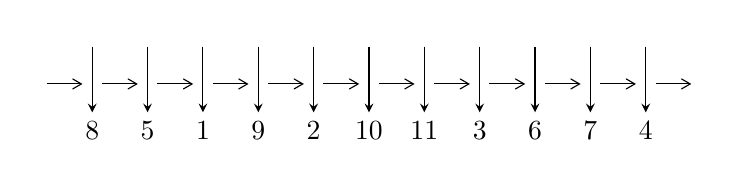
\begin{tikzpicture}[x=20pt, y=17pt]
	% nodes
	\node (C0) at (0, 0) {};
	\node (C1) at (1, 0) {};
	\node (C1U) at (1, +1) {};
	\node (C1D) at (1, -1) {8};

	\node (C2) at (2, 0) {};
	\node (C2U) at (2, +1) {};
	\node (C2D) at (2, -1) {5};

	\node (C3) at (3, 0) {};
	\node (C3U) at (3, +1) {};
	\node (C3D) at (3, -1) {1};

	\node (C4) at (4, 0) {};
	\node (C4U) at (4, +1) {};
	\node (C4D) at (4, -1) {9};

	\node (C5) at (5, 0) {};
	\node (C5U) at (5, +1) {};
	\node (C5D) at (5, -1) {2};

	\node (C6) at (6, 0) {};
	\node (C6U) at (6, +1) {};
	\node (C6D) at (6, -1) {10};

	\node (C7) at (7, 0) {};
	\node (C7U) at (7, +1) {};
	\node (C7D) at (7, -1) {11};

	\node (C8) at (8, 0) {};
	\node (C8U) at (8, +1) {};
	\node (C8D) at (8, -1) {3};

	\node (C9) at (9, 0) {};
	\node (C9U) at (9, +1) {};
	\node (C9D) at (9, -1) {6};

	\node (C10) at (10, 0) {};
	\node (C10U) at (10, +1) {};
	\node (C10D) at (10, -1) {7};

	\node (C11) at (11, 0) {};
	\node (C11U) at (11, +1) {};
	\node (C11D) at (11, -1) {4};
	\node (C12) at (12, 0) {};

	% arrows
	\draw[->,>={angle 60}]
	(C0) edge (C1) (C1) edge (C2) (C2) edge (C3) (C3) edge (C4) (C4) edge (C5) (C5) edge (C6) (C6) edge (C7) (C7) edge (C8) (C8) edge (C9) (C9) edge (C10) (C10) edge (C11) (C11) edge (C12) ;	\draw[->,>=stealth]
	(C1U) edge (C1D) (C2U) edge (C2D) (C3U) edge (C3D) (C4U) edge (C4D) (C5U) edge (C5D) (C6U) edge (C6D) (C7U) edge (C7D) (C8U) edge (C8D) (C9U) edge (C9D) (C10U) edge (C10D) (C11U) edge (C11D) ;
	\end{tikzpicture} \\
\hhline{~~} \\& 
\textbf{Solving Sequence} \\ \cline{2-2} 
 &
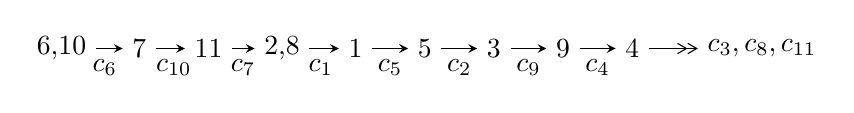
\begin{tikzpicture}[x=25pt, y=7pt]
	% node
	\node (A0) at (-1/8, 0) {6,10};
	\node (A1) at (1, 0) {7};
	\node (A2) at (2, 0) {11};
	\node (A3) at (49/16, 0) {2,8};
	\node (A4) at (33/8, 0) {1};
	\node (A5) at (41/8, 0) {5};
	\node (A6) at (49/8, 0) {3};
	\node (A7) at (57/8, 0) {9};
	\node (A8) at (65/8, 0) {4};
	\node (C1) at (1/2, -1) {$c_{6}$};
	\node (C2) at (3/2, -1) {$c_{10}$};
	\node (C3) at (5/2, -1) {$c_{7}$};
	\node (C4) at (29/8, -1) {$c_{1}$};
	\node (C5) at (37/8, -1) {$c_{5}$};
	\node (C6) at (45/8, -1) {$c_{2}$};
	\node (C7) at (53/8, -1) {$c_{9}$};
	\node (C8) at (61/8, -1) {$c_{4}$};
	\node (A9) at (10, 0) {$c_{3},c_{8},c_{11}$};

	% edge
	\draw[->,>=stealth]	
	(A0) edge (A1) (A1) edge (A2) (A2) edge (A3) (A3) edge (A4) (A4) edge (A5) (A5) edge (A6) (A6) edge (A7) (A7) edge (A8) ;
	\draw[->>,>={angle 60}]	
	(A8) edge (A9);
\end{tikzpicture} \\ 

\end{tabular} \\

\footnotetext{
The image of knot diagram is generated by the software ``\textbf{Draw programme}" developed by Andrew Bartholomew(\url{http://www.layer8.co.uk/maths/draw/index.htm\#Running-draw}), where we modified some parts for our purpose(\url{https://github.com/CATsTAILs/LinksPainter}).
}\phantom \\ \newline 
\centering \textbf{Ideals for irreducible components\footnotemark of $X_{\text{par}}$} 
 
\begin{align*}
I^u_{1}&=\langle 
9320183 u^{20}-5745909 u^{19}+\cdots+120011978 b-47600802,\\
\phantom{I^u_{1}}&\phantom{= \langle  }49214757 u^{20}-69440884 u^{19}+\cdots+240023956 a+223258849,\;u^{21}-2 u^{20}+\cdots+13 u-4\rangle \\
I^u_{2}&=\langle 
- u^{15} a-3 u^{15}+\cdots+3 a-1,\;-4 u^{15} a+18 u^{15}+\cdots-6 a+36,\\
\phantom{I^u_{2}}&\phantom{= \langle  }u^{16}- u^{15}-9 u^{14}+8 u^{13}+31 u^{12}-22 u^{11}-52 u^{10}+22 u^9+47 u^8-2 u^7-24 u^6-6 u^5+2 u^4+6 u^3+2 u^2-1\rangle \\
I^u_{3}&=\langle 
b+1,\;2 a+3,\;u^2+u-1\rangle \\
I^u_{4}&=\langle 
b- a-1,\;a^2+2 a+2,\;u-1\rangle \\
\\
\end{align*}
\raggedright * 4 irreducible components of $\dim_{\mathbb{C}}=0$, with total 57 representations.\\
\footnotetext{All coefficients of polynomials are rational numbers. But the coefficients are sometimes approximated in decimal forms when there is not enough margin.}
\newpage
\renewcommand{\arraystretch}{1}
\centering \section*{I. $I^u_{1}= \langle 9.32\times10^{6} u^{20}-5.75\times10^{6} u^{19}+\cdots+1.20\times10^{8} b-4.76\times10^{7},\;4.92\times10^{7} u^{20}-6.94\times10^{7} u^{19}+\cdots+2.40\times10^{8} a+2.23\times10^{8},\;u^{21}-2 u^{20}+\cdots+13 u-4 \rangle$}
\flushleft \textbf{(i) Arc colorings}\\
\begin{tabular}{m{7pt} m{180pt} m{7pt} m{180pt} }
\flushright $a_{6}=$&$\begin{pmatrix}1\\0\end{pmatrix}$ \\
\flushright $a_{10}=$&$\begin{pmatrix}0\\u\end{pmatrix}$ \\
\flushright $a_{7}=$&$\begin{pmatrix}1\\u^2\end{pmatrix}$ \\
\flushright $a_{11}=$&$\begin{pmatrix}- u\\- u^3+u\end{pmatrix}$ \\
\flushright $a_{2}=$&$\begin{pmatrix}-0.205041 u^{20}+0.289308 u^{19}+\cdots-1.57998 u-0.930152\\-0.0776604 u^{20}+0.0478778 u^{19}+\cdots-0.825434 u+0.396634\end{pmatrix}$ \\
\flushright $a_{8}=$&$\begin{pmatrix}- u^2+1\\- u^4+2 u^2\end{pmatrix}$ \\
\flushright $a_{1}=$&$\begin{pmatrix}-0.222415 u^{20}+0.221463 u^{19}+\cdots-0.915430 u-0.633782\\-0.230117 u^{20}+0.198897 u^{19}+\cdots+0.482667 u-0.0496061\end{pmatrix}$ \\
\flushright $a_{5}=$&$\begin{pmatrix}0.210965 u^{20}-0.285506 u^{19}+\cdots+1.46088 u+1.21110\\0.145840 u^{20}-0.137084 u^{19}+\cdots+1.32796 u-0.343964\end{pmatrix}$ \\
\flushright $a_{3}=$&$\begin{pmatrix}-0.399042 u^{20}+0.523770 u^{19}+\cdots-1.95821 u-1.41205\\-0.279364 u^{20}+0.259774 u^{19}+\cdots-1.80557 u+0.498910\end{pmatrix}$ \\
\flushright $a_{9}=$&$\begin{pmatrix}u\\u\end{pmatrix}$ \\
\flushright $a_{4}=$&$\begin{pmatrix}0.219932 u^{20}-0.302643 u^{19}+\cdots+0.964152 u+1.28379\\0.154807 u^{20}-0.154222 u^{19}+\cdots+0.831233 u-0.271279\end{pmatrix}$\\ \flushright $a_{4}=$&$\begin{pmatrix}0.219932 u^{20}-0.302643 u^{19}+\cdots+0.964152 u+1.28379\\0.154807 u^{20}-0.154222 u^{19}+\cdots+0.831233 u-0.271279\end{pmatrix}$\\&\end{tabular}
\flushleft \textbf{(ii) Obstruction class $= -1$}\\~\\
\flushleft \textbf{(iii) Cusp Shapes $= \frac{162514487}{240023956} u^{20}-\frac{304511969}{240023956} u^{19}+\cdots+\frac{520499563}{60005989} u-\frac{1134730210}{60005989}$}\\~\\
\newpage\renewcommand{\arraystretch}{1}
\flushleft \textbf{(iv) u-Polynomials at the component}\newline \\
\begin{tabular}{m{50pt}|m{274pt}}
Crossings & \hspace{64pt}u-Polynomials at each crossing \\
\hline $$\begin{aligned}c_{1},c_{4}\end{aligned}$$&$\begin{aligned}
&4(4 u^{21}-2 u^{20}+\cdots+6 u+2)
\end{aligned}$\\
\hline $$\begin{aligned}c_{2},c_{3},c_{5}\\c_{11}\end{aligned}$$&$\begin{aligned}
&u^{21}+2 u^{20}+\cdots+5 u+1
\end{aligned}$\\
\hline $$\begin{aligned}c_{6},c_{7},c_{9}\\c_{10}\end{aligned}$$&$\begin{aligned}
&u^{21}+2 u^{20}+\cdots+13 u+4
\end{aligned}$\\
\hline $$\begin{aligned}c_{8}\end{aligned}$$&$\begin{aligned}
&u^{21}+3 u^{20}+\cdots+88 u+32
\end{aligned}$\\
\hline
\end{tabular}\\~\\
\newpage\renewcommand{\arraystretch}{1}
\flushleft \textbf{(v) Riley Polynomials at the component}\newline \\
\begin{tabular}{m{50pt}|m{274pt}}
Crossings & \hspace{64pt}Riley Polynomials at each crossing \\
\hline $$\begin{aligned}c_{1},c_{4}\end{aligned}$$&$\begin{aligned}
&16(16 y^{21}-76 y^{20}+\cdots+76 y-4)
\end{aligned}$\\
\hline $$\begin{aligned}c_{2},c_{3},c_{5}\\c_{11}\end{aligned}$$&$\begin{aligned}
&y^{21}+8 y^{20}+\cdots+5 y-1
\end{aligned}$\\
\hline $$\begin{aligned}c_{6},c_{7},c_{9}\\c_{10}\end{aligned}$$&$\begin{aligned}
&y^{21}-24 y^{20}+\cdots+273 y-16
\end{aligned}$\\
\hline $$\begin{aligned}c_{8}\end{aligned}$$&$\begin{aligned}
&y^{21}+7 y^{20}+\cdots+448 y-1024
\end{aligned}$\\
\hline
\end{tabular}\\~\\
\newpage\flushleft \textbf{(vi) Complex Volumes and Cusp Shapes}
$$\begin{array}{c|c|c}  
\text{Solutions to }I^u_{1}& \I (\text{vol} + \sqrt{-1}CS) & \text{Cusp shape}\\
 \hline 
\begin{aligned}
u &= -0.789797 + 0.624633 I \\
a &= -1.51457 - 0.44640 I \\
b &= -0.546053 + 1.249230 I\end{aligned}
 & \phantom{-}3.68387 + 11.47460 I & -9.39826 - 8.82846 I \\ \hline\begin{aligned}
u &= -0.789797 - 0.624633 I \\
a &= -1.51457 + 0.44640 I \\
b &= -0.546053 - 1.249230 I\end{aligned}
 & \phantom{-}3.68387 - 11.47460 I & -9.39826 + 8.82846 I \\ \hline\begin{aligned}
u &= \phantom{-}0.758227 + 0.411195 I \\
a &= -0.698370 + 0.278847 I \\
b &= \phantom{-}0.041928 - 0.594017 I\end{aligned}
 & -0.315718 - 0.478711 I & -14.5208 + 0.8983 I \\ \hline\begin{aligned}
u &= \phantom{-}0.758227 - 0.411195 I \\
a &= -0.698370 - 0.278847 I \\
b &= \phantom{-}0.041928 + 0.594017 I\end{aligned}
 & -0.315718 + 0.478711 I & -14.5208 - 0.8983 I \\ \hline\begin{aligned}
u &= -0.179300 + 0.815897 I \\
a &= \phantom{-}0.030732 + 0.642646 I \\
b &= -0.442140 - 1.177470 I\end{aligned}
 & \phantom{-}5.53762 - 6.70880 I & -6.60250 + 5.49950 I \\ \hline\begin{aligned}
u &= -0.179300 - 0.815897 I \\
a &= \phantom{-}0.030732 - 0.642646 I \\
b &= -0.442140 + 1.177470 I\end{aligned}
 & \phantom{-}5.53762 + 6.70880 I & -6.60250 - 5.49950 I \\ \hline\begin{aligned}
u &= \phantom{-}0.506129 + 0.654446 I \\
a &= \phantom{-}0.657349 - 1.025090 I \\
b &= \phantom{-}0.372085 + 0.842002 I\end{aligned}
 & \phantom{-}0.34108 - 3.49247 I & -11.9725 + 8.3783 I \\ \hline\begin{aligned}
u &= \phantom{-}0.506129 - 0.654446 I \\
a &= \phantom{-}0.657349 + 1.025090 I \\
b &= \phantom{-}0.372085 - 0.842002 I\end{aligned}
 & \phantom{-}0.34108 + 3.49247 I & -11.9725 - 8.3783 I \\ \hline\begin{aligned}
u &= \phantom{-}1.209060 + 0.446540 I \\
a &= \phantom{-}0.070327 + 0.349474 I \\
b &= -0.345184 + 1.020620 I\end{aligned}
 & \phantom{-}1.29592 + 2.27858 I & -10.67873 - 5.63740 I \\ \hline\begin{aligned}
u &= \phantom{-}1.209060 - 0.446540 I \\
a &= \phantom{-}0.070327 - 0.349474 I \\
b &= -0.345184 - 1.020620 I\end{aligned}
 & \phantom{-}1.29592 - 2.27858 I & -10.67873 + 5.63740 I\\
 \hline 
 \end{array}$$\newpage$$\begin{array}{c|c|c}  
\text{Solutions to }I^u_{1}& \I (\text{vol} + \sqrt{-1}CS) & \text{Cusp shape}\\
 \hline 
\begin{aligned}
u &= -0.639776 + 0.168175 I \\
a &= \phantom{-}1.34866 + 0.57840 I \\
b &= \phantom{-}1.079910 + 0.285594 I\end{aligned}
 & -2.83019 + 0.37915 I & -14.9029 - 12.5783 I \\ \hline\begin{aligned}
u &= -0.639776 - 0.168175 I \\
a &= \phantom{-}1.34866 - 0.57840 I \\
b &= \phantom{-}1.079910 - 0.285594 I\end{aligned}
 & -2.83019 - 0.37915 I & -14.9029 + 12.5783 I \\ \hline\begin{aligned}
u &= -1.56702 + 0.20612 I \\
a &= \phantom{-}1.206150 + 0.091091 I \\
b &= \phantom{-}0.510228 - 1.044980 I\end{aligned}
 & -6.63082 + 6.65001 I & -13.3056 - 6.2387 I \\ \hline\begin{aligned}
u &= -1.56702 - 0.20612 I \\
a &= \phantom{-}1.206150 - 0.091091 I \\
b &= \phantom{-}0.510228 + 1.044980 I\end{aligned}
 & -6.63082 - 6.65001 I & -13.3056 + 6.2387 I \\ \hline\begin{aligned}
u &= \phantom{-}1.59922 + 0.05529 I \\
a &= \phantom{-}1.76881 - 0.60078 I \\
b &= \phantom{-}1.291780 - 0.473779 I\end{aligned}
 & -10.58370 - 1.26080 I & -14.0233 + 4.6800 I \\ \hline\begin{aligned}
u &= \phantom{-}1.59922 - 0.05529 I \\
a &= \phantom{-}1.76881 + 0.60078 I \\
b &= \phantom{-}1.291780 + 0.473779 I\end{aligned}
 & -10.58370 + 1.26080 I & -14.0233 - 4.6800 I \\ \hline\begin{aligned}
u &= \phantom{-}1.63963 + 0.18902 I \\
a &= -1.69792 - 0.35423 I \\
b &= -0.63892 - 1.29044 I\end{aligned}
 & -4.5325 - 14.5799 I & -12.0752 + 7.7299 I \\ \hline\begin{aligned}
u &= \phantom{-}1.63963 - 0.18902 I \\
a &= -1.69792 + 0.35423 I \\
b &= -0.63892 + 1.29044 I\end{aligned}
 & -4.5325 + 14.5799 I & -12.0752 - 7.7299 I \\ \hline\begin{aligned}
u &= -1.68983 + 0.00575 I \\
a &= -0.819332 - 0.396829 I \\
b &= -0.450400 - 0.614576 I\end{aligned}
 & -9.51673 - 1.46421 I & -13.5665 + 4.8534 I \\ \hline\begin{aligned}
u &= -1.68983 - 0.00575 I \\
a &= -0.819332 + 0.396829 I \\
b &= -0.450400 + 0.614576 I\end{aligned}
 & -9.51673 + 1.46421 I & -13.5665 - 4.8534 I\\
 \hline 
 \end{array}$$\newpage$$\begin{array}{c|c|c}  
\text{Solutions to }I^u_{1}& \I (\text{vol} + \sqrt{-1}CS) & \text{Cusp shape}\\
 \hline 
\begin{aligned}
u &= \phantom{-}0.306916\phantom{ +0.000000I} \\
a &= -0.953646\phantom{ +0.000000I} \\
b &= \phantom{-}0.253532\phantom{ +0.000000I}\end{aligned}
 & -0.600717\phantom{ +0.000000I} & -16.6570\phantom{ +0.000000I}\\
 \hline 
 \end{array}$$\newpage\newpage\renewcommand{\arraystretch}{1}
\centering \section*{II. $I^u_{2}= \langle - u^{15} a-3 u^{15}+\cdots+3 a-1,\;-4 u^{15} a+18 u^{15}+\cdots-6 a+36,\;u^{16}- u^{15}+\cdots+2 u^2-1 \rangle$}
\flushleft \textbf{(i) Arc colorings}\\
\begin{tabular}{m{7pt} m{180pt} m{7pt} m{180pt} }
\flushright $a_{6}=$&$\begin{pmatrix}1\\0\end{pmatrix}$ \\
\flushright $a_{10}=$&$\begin{pmatrix}0\\u\end{pmatrix}$ \\
\flushright $a_{7}=$&$\begin{pmatrix}1\\u^2\end{pmatrix}$ \\
\flushright $a_{11}=$&$\begin{pmatrix}- u\\- u^3+u\end{pmatrix}$ \\
\flushright $a_{2}=$&$\begin{pmatrix}a\\\frac{1}{2} u^{15} a+\frac{3}{2} u^{15}+\cdots-\frac{3}{2} a+\frac{1}{2}\end{pmatrix}$ \\
\flushright $a_{8}=$&$\begin{pmatrix}- u^2+1\\- u^4+2 u^2\end{pmatrix}$ \\
\flushright $a_{1}=$&$\begin{pmatrix}u^{15} a+2 u^{15}+\cdots- a+1\\\frac{1}{2} u^{15} a+\frac{3}{2} u^{15}+\cdots-\frac{1}{2} a+\frac{1}{2}\end{pmatrix}$ \\
\flushright $a_{5}=$&$\begin{pmatrix}\frac{3}{2} u^{15} a-\frac{7}{2} u^{15}+\cdots+\frac{1}{2} a-\frac{11}{2}\\-\frac{1}{2} u^{15} a+\frac{1}{2} u^{15}+\cdots-\frac{1}{2} a-\frac{1}{2}\end{pmatrix}$ \\
\flushright $a_{3}=$&$\begin{pmatrix}- u^{15}+8 u^{13}-22 u^{11}+22 u^9-2 u^7-6 u^5+6 u^3\\- u^{15}+9 u^{13}-30 u^{11}+45 u^9-30 u^7+8 u^5+2 u^3- u\end{pmatrix}$ \\
\flushright $a_{9}=$&$\begin{pmatrix}u\\u\end{pmatrix}$ \\
\flushright $a_{4}=$&$\begin{pmatrix}\frac{3}{2} u^{15} a-\frac{5}{2} u^{15}+\cdots+\frac{1}{2} a-\frac{5}{2}\\-\frac{1}{2} u^{15} a+\frac{3}{2} u^{15}+\cdots-\frac{1}{2} a+\frac{5}{2}\end{pmatrix}$\\ \flushright $a_{4}=$&$\begin{pmatrix}\frac{3}{2} u^{15} a-\frac{5}{2} u^{15}+\cdots+\frac{1}{2} a-\frac{5}{2}\\-\frac{1}{2} u^{15} a+\frac{3}{2} u^{15}+\cdots-\frac{1}{2} a+\frac{5}{2}\end{pmatrix}$\\&\end{tabular}
\flushleft \textbf{(ii) Obstruction class $= -1$}\\~\\
\flushleft \textbf{(iii) Cusp Shapes $= 4 u^{13}-32 u^{11}+92 u^9+4 u^8-112 u^7-20 u^6+56 u^5+28 u^4-12 u^3-8 u^2-12 u-10$}\\~\\
\newpage\renewcommand{\arraystretch}{1}
\flushleft \textbf{(iv) u-Polynomials at the component}\newline \\
\begin{tabular}{m{50pt}|m{274pt}}
Crossings & \hspace{64pt}u-Polynomials at each crossing \\
\hline $$\begin{aligned}c_{1},c_{4}\end{aligned}$$&$\begin{aligned}
&u^{32}-3 u^{31}+\cdots+52 u+17
\end{aligned}$\\
\hline $$\begin{aligned}c_{2},c_{3},c_{5}\\c_{11}\end{aligned}$$&$\begin{aligned}
&u^{32}-5 u^{31}+\cdots-11 u+2
\end{aligned}$\\
\hline $$\begin{aligned}c_{6},c_{7},c_{9}\\c_{10}\end{aligned}$$&$\begin{aligned}
&(u^{16}+u^{15}+\cdots+2 u^2-1)^{2}
\end{aligned}$\\
\hline $$\begin{aligned}c_{8}\end{aligned}$$&$\begin{aligned}
&(u^{16}- u^{15}+\cdots+2 u-1)^{2}
\end{aligned}$\\
\hline
\end{tabular}\\~\\
\newpage\renewcommand{\arraystretch}{1}
\flushleft \textbf{(v) Riley Polynomials at the component}\newline \\
\begin{tabular}{m{50pt}|m{274pt}}
Crossings & \hspace{64pt}Riley Polynomials at each crossing \\
\hline $$\begin{aligned}c_{1},c_{4}\end{aligned}$$&$\begin{aligned}
&y^{32}+11 y^{31}+\cdots+14534 y+289
\end{aligned}$\\
\hline $$\begin{aligned}c_{2},c_{3},c_{5}\\c_{11}\end{aligned}$$&$\begin{aligned}
&y^{32}+19 y^{31}+\cdots+59 y+4
\end{aligned}$\\
\hline $$\begin{aligned}c_{6},c_{7},c_{9}\\c_{10}\end{aligned}$$&$\begin{aligned}
&(y^{16}-19 y^{15}+\cdots-4 y+1)^{2}
\end{aligned}$\\
\hline $$\begin{aligned}c_{8}\end{aligned}$$&$\begin{aligned}
&(y^{16}+5 y^{15}+\cdots-4 y+1)^{2}
\end{aligned}$\\
\hline
\end{tabular}\\~\\
\newpage\flushleft \textbf{(vi) Complex Volumes and Cusp Shapes}
$$\begin{array}{c|c|c}  
\text{Solutions to }I^u_{2}& \I (\text{vol} + \sqrt{-1}CS) & \text{Cusp shape}\\
 \hline 
\begin{aligned}
u &= -0.752457 + 0.456573 I \\
a &= -0.862515 - 0.499116 I \\
b &= -0.965256 - 0.143588 I\end{aligned}
 & \phantom{-}0.28749 + 6.07197 I & -12.6157 - 7.0281 I \\ \hline\begin{aligned}
u &= -0.752457 + 0.456573 I \\
a &= \phantom{-}1.61525 + 0.23701 I \\
b &= \phantom{-}0.562596 - 1.228100 I\end{aligned}
 & \phantom{-}0.28749 + 6.07197 I & -12.6157 - 7.0281 I \\ \hline\begin{aligned}
u &= -0.752457 - 0.456573 I \\
a &= -0.862515 + 0.499116 I \\
b &= -0.965256 + 0.143588 I\end{aligned}
 & \phantom{-}0.28749 - 6.07197 I & -12.6157 + 7.0281 I \\ \hline\begin{aligned}
u &= -0.752457 - 0.456573 I \\
a &= \phantom{-}1.61525 - 0.23701 I \\
b &= \phantom{-}0.562596 + 1.228100 I\end{aligned}
 & \phantom{-}0.28749 - 6.07197 I & -12.6157 + 7.0281 I \\ \hline\begin{aligned}
u &= \phantom{-}0.790211 + 0.368636 I \\
a &= -0.861711 - 0.010777 I \\
b &= \phantom{-}0.058639 - 0.741860 I\end{aligned}
 & -0.311107 - 0.489680 I & -14.3561 + 1.4314 I \\ \hline\begin{aligned}
u &= \phantom{-}0.790211 + 0.368636 I \\
a &= -0.580679 + 0.527896 I \\
b &= -0.071737 - 0.398232 I\end{aligned}
 & -0.311107 - 0.489680 I & -14.3561 + 1.4314 I \\ \hline\begin{aligned}
u &= \phantom{-}0.790211 - 0.368636 I \\
a &= -0.861711 + 0.010777 I \\
b &= \phantom{-}0.058639 + 0.741860 I\end{aligned}
 & -0.311107 + 0.489680 I & -14.3561 - 1.4314 I \\ \hline\begin{aligned}
u &= \phantom{-}0.790211 - 0.368636 I \\
a &= -0.580679 - 0.527896 I \\
b &= -0.071737 + 0.398232 I\end{aligned}
 & -0.311107 + 0.489680 I & -14.3561 - 1.4314 I \\ \hline\begin{aligned}
u &= -0.452620 + 0.425410 I \\
a &= \phantom{-}0.223204 - 0.029590 I \\
b &= -0.325222 - 1.319700 I\end{aligned}
 & \phantom{-}5.17692 + 1.52971 I & -5.27263 - 5.08772 I \\ \hline\begin{aligned}
u &= -0.452620 + 0.425410 I \\
a &= -2.28305 - 0.32185 I \\
b &= -0.511738 + 1.137200 I\end{aligned}
 & \phantom{-}5.17692 + 1.52971 I & -5.27263 - 5.08772 I\\
 \hline 
 \end{array}$$\newpage$$\begin{array}{c|c|c}  
\text{Solutions to }I^u_{2}& \I (\text{vol} + \sqrt{-1}CS) & \text{Cusp shape}\\
 \hline 
\begin{aligned}
u &= -0.452620 - 0.425410 I \\
a &= \phantom{-}0.223204 + 0.029590 I \\
b &= -0.325222 + 1.319700 I\end{aligned}
 & \phantom{-}5.17692 - 1.52971 I & -5.27263 + 5.08772 I \\ \hline\begin{aligned}
u &= -0.452620 - 0.425410 I \\
a &= -2.28305 + 0.32185 I \\
b &= -0.511738 - 1.137200 I\end{aligned}
 & \phantom{-}5.17692 - 1.52971 I & -5.27263 + 5.08772 I \\ \hline\begin{aligned}
u &= -0.071750 + 0.572783 I \\
a &= -0.393981 - 0.880662 I \\
b &= \phantom{-}0.338699 + 1.140160 I\end{aligned}
 & \phantom{-}2.27257 - 2.57669 I & -8.69244 + 2.71681 I \\ \hline\begin{aligned}
u &= -0.071750 + 0.572783 I \\
a &= -0.152598 - 0.881762 I \\
b &= -0.658604 + 0.021898 I\end{aligned}
 & \phantom{-}2.27257 - 2.57669 I & -8.69244 + 2.71681 I \\ \hline\begin{aligned}
u &= -0.071750 - 0.572783 I \\
a &= -0.393981 + 0.880662 I \\
b &= \phantom{-}0.338699 - 1.140160 I\end{aligned}
 & \phantom{-}2.27257 + 2.57669 I & -8.69244 - 2.71681 I \\ \hline\begin{aligned}
u &= -0.071750 - 0.572783 I \\
a &= -0.152598 + 0.881762 I \\
b &= -0.658604 - 0.021898 I\end{aligned}
 & \phantom{-}2.27257 + 2.57669 I & -8.69244 - 2.71681 I \\ \hline\begin{aligned}
u &= \phantom{-}0.508466\phantom{ +0.000000I} \\
a &= \phantom{-}6.38440 + 5.02047 I \\
b &= \phantom{-}0.074040 - 1.008190 I\end{aligned}
 & \phantom{-}2.52578\phantom{ +0.000000I} & -17.0940\phantom{ +0.000000I} \\ \hline\begin{aligned}
u &= \phantom{-}0.508466\phantom{ +0.000000I} \\
a &= \phantom{-}6.38440 - 5.02047 I \\
b &= \phantom{-}0.074040 + 1.008190 I\end{aligned}
 & \phantom{-}2.52578\phantom{ +0.000000I} & -17.0940\phantom{ +0.000000I} \\ \hline\begin{aligned}
u &= \phantom{-}1.52559 + 0.07425 I \\
a &= -0.185891 + 0.863663 I \\
b &= -0.18841 + 1.53021 I\end{aligned}
 & -1.40970 - 3.12434 I & -9.94060 + 3.66013 I \\ \hline\begin{aligned}
u &= \phantom{-}1.52559 + 0.07425 I \\
a &= -1.91032 - 0.81582 I \\
b &= -0.793946 - 1.008570 I\end{aligned}
 & -1.40970 - 3.12434 I & -9.94060 + 3.66013 I\\
 \hline 
 \end{array}$$\newpage$$\begin{array}{c|c|c}  
\text{Solutions to }I^u_{2}& \I (\text{vol} + \sqrt{-1}CS) & \text{Cusp shape}\\
 \hline 
\begin{aligned}
u &= \phantom{-}1.52559 - 0.07425 I \\
a &= -0.185891 - 0.863663 I \\
b &= -0.18841 - 1.53021 I\end{aligned}
 & -1.40970 + 3.12434 I & -9.94060 - 3.66013 I \\ \hline\begin{aligned}
u &= \phantom{-}1.52559 - 0.07425 I \\
a &= -1.91032 + 0.81582 I \\
b &= -0.793946 + 1.008570 I\end{aligned}
 & -1.40970 + 3.12434 I & -9.94060 - 3.66013 I \\ \hline\begin{aligned}
u &= -1.57280\phantom{ +0.000000I} \\
a &= \phantom{-}1.97074 + 0.61509 I \\
b &= \phantom{-}0.237438 - 1.081260 I\end{aligned}
 & -4.71670\phantom{ +0.000000I} & -16.1480\phantom{ +0.000000I} \\ \hline\begin{aligned}
u &= -1.57280\phantom{ +0.000000I} \\
a &= \phantom{-}1.97074 - 0.61509 I \\
b &= \phantom{-}0.237438 + 1.081260 I\end{aligned}
 & -4.71670\phantom{ +0.000000I} & -16.1480\phantom{ +0.000000I} \\ \hline\begin{aligned}
u &= \phantom{-}1.62338 + 0.13130 I \\
a &= -1.49404 + 0.52581 I \\
b &= -1.144250 + 0.248239 I\end{aligned}
 & -7.82454 - 8.28859 I & -14.5771 + 5.2713 I \\ \hline\begin{aligned}
u &= \phantom{-}1.62338 + 0.13130 I \\
a &= \phantom{-}1.68539 + 0.55122 I \\
b &= \phantom{-}0.72433 + 1.27550 I\end{aligned}
 & -7.82454 - 8.28859 I & -14.5771 + 5.2713 I \\ \hline\begin{aligned}
u &= \phantom{-}1.62338 - 0.13130 I \\
a &= -1.49404 - 0.52581 I \\
b &= -1.144250 - 0.248239 I\end{aligned}
 & -7.82454 + 8.28859 I & -14.5771 - 5.2713 I \\ \hline\begin{aligned}
u &= \phantom{-}1.62338 - 0.13130 I \\
a &= \phantom{-}1.68539 - 0.55122 I \\
b &= \phantom{-}0.72433 - 1.27550 I\end{aligned}
 & -7.82454 + 8.28859 I & -14.5771 - 5.2713 I \\ \hline\begin{aligned}
u &= -1.63018 + 0.10414 I \\
a &= -1.297790 + 0.134879 I \\
b &= -0.436027 + 0.931326 I\end{aligned}
 & -8.61070 + 2.28357 I & -15.9247 - 0.3083 I \\ \hline\begin{aligned}
u &= -1.63018 + 0.10414 I \\
a &= \phantom{-}0.643588 + 0.194017 I \\
b &= \phantom{-}0.599447 + 0.332807 I\end{aligned}
 & -8.61070 + 2.28357 I & -15.9247 - 0.3083 I\\
 \hline 
 \end{array}$$\newpage$$\begin{array}{c|c|c}  
\text{Solutions to }I^u_{2}& \I (\text{vol} + \sqrt{-1}CS) & \text{Cusp shape}\\
 \hline 
\begin{aligned}
u &= -1.63018 - 0.10414 I \\
a &= -1.297790 - 0.134879 I \\
b &= -0.436027 - 0.931326 I\end{aligned}
 & -8.61070 - 2.28357 I & -15.9247 + 0.3083 I \\ \hline\begin{aligned}
u &= -1.63018 - 0.10414 I \\
a &= \phantom{-}0.643588 - 0.194017 I \\
b &= \phantom{-}0.599447 - 0.332807 I\end{aligned}
 & -8.61070 - 2.28357 I & -15.9247 + 0.3083 I\\
 \hline 
 \end{array}$$\newpage\newpage\renewcommand{\arraystretch}{1}
\centering \section*{III. $I^u_{3}= \langle b+1,\;2 a+3,\;u^2+u-1 \rangle$}
\flushleft \textbf{(i) Arc colorings}\\
\begin{tabular}{m{7pt} m{180pt} m{7pt} m{180pt} }
\flushright $a_{6}=$&$\begin{pmatrix}1\\0\end{pmatrix}$ \\
\flushright $a_{10}=$&$\begin{pmatrix}0\\u\end{pmatrix}$ \\
\flushright $a_{7}=$&$\begin{pmatrix}1\\- u+1\end{pmatrix}$ \\
\flushright $a_{11}=$&$\begin{pmatrix}- u\\- u+1\end{pmatrix}$ \\
\flushright $a_{2}=$&$\begin{pmatrix}-1.5\\-1\end{pmatrix}$ \\
\flushright $a_{8}=$&$\begin{pmatrix}u\\u\end{pmatrix}$ \\
\flushright $a_{1}=$&$\begin{pmatrix}-\frac{1}{2} u-1\\-\frac{1}{2} u-\frac{1}{2}\end{pmatrix}$ \\
\flushright $a_{5}=$&$\begin{pmatrix}-0.5\\-1\end{pmatrix}$ \\
\flushright $a_{3}=$&$\begin{pmatrix}-2\\-2\end{pmatrix}$ \\
\flushright $a_{9}=$&$\begin{pmatrix}u\\u\end{pmatrix}$ \\
\flushright $a_{4}=$&$\begin{pmatrix}\frac{1}{2} u-1\\\frac{1}{2} u-\frac{3}{2}\end{pmatrix}$\\ \flushright $a_{4}=$&$\begin{pmatrix}\frac{1}{2} u-1\\\frac{1}{2} u-\frac{3}{2}\end{pmatrix}$\\&\end{tabular}
\flushleft \textbf{(ii) Obstruction class $= 1$}\\~\\
\flushleft \textbf{(iii) Cusp Shapes $= \frac{15}{4} u-\frac{39}{4}$}\\~\\
\newpage\renewcommand{\arraystretch}{1}
\flushleft \textbf{(iv) u-Polynomials at the component}\newline \\
\begin{tabular}{m{50pt}|m{274pt}}
Crossings & \hspace{64pt}u-Polynomials at each crossing \\
\hline $$\begin{aligned}c_{1}\end{aligned}$$&$\begin{aligned}
&4(4 u^2-2 u-1)
\end{aligned}$\\
\hline $$\begin{aligned}c_{2},c_{11}\end{aligned}$$&$\begin{aligned}
&(u-1)^2
\end{aligned}$\\
\hline $$\begin{aligned}c_{3},c_{5}\end{aligned}$$&$\begin{aligned}
&(u+1)^2
\end{aligned}$\\
\hline $$\begin{aligned}c_{4}\end{aligned}$$&$\begin{aligned}
&4(4 u^2+2 u-1)
\end{aligned}$\\
\hline $$\begin{aligned}c_{6},c_{7}\end{aligned}$$&$\begin{aligned}
&u^2+u-1
\end{aligned}$\\
\hline $$\begin{aligned}c_{8}\end{aligned}$$&$\begin{aligned}
&u^2
\end{aligned}$\\
\hline $$\begin{aligned}c_{9},c_{10}\end{aligned}$$&$\begin{aligned}
&u^2- u-1
\end{aligned}$\\
\hline
\end{tabular}\\~\\
\newpage\renewcommand{\arraystretch}{1}
\flushleft \textbf{(v) Riley Polynomials at the component}\newline \\
\begin{tabular}{m{50pt}|m{274pt}}
Crossings & \hspace{64pt}Riley Polynomials at each crossing \\
\hline $$\begin{aligned}c_{1},c_{4}\end{aligned}$$&$\begin{aligned}
&16(16 y^2-12 y+1)
\end{aligned}$\\
\hline $$\begin{aligned}c_{2},c_{3},c_{5}\\c_{11}\end{aligned}$$&$\begin{aligned}
&(y-1)^2
\end{aligned}$\\
\hline $$\begin{aligned}c_{6},c_{7},c_{9}\\c_{10}\end{aligned}$$&$\begin{aligned}
&y^2-3 y+1
\end{aligned}$\\
\hline $$\begin{aligned}c_{8}\end{aligned}$$&$\begin{aligned}
&y^2
\end{aligned}$\\
\hline
\end{tabular}\\~\\
\newpage\flushleft \textbf{(vi) Complex Volumes and Cusp Shapes}
$$\begin{array}{c|c|c}  
\text{Solutions to }I^u_{3}& \I (\text{vol} + \sqrt{-1}CS) & \text{Cusp shape}\\
 \hline 
\begin{aligned}
u &= \phantom{-}0.618034\phantom{ +0.000000I} \\
a &= -1.50000\phantom{ +0.000000I} \\
b &= -1.00000\phantom{ +0.000000I}\end{aligned}
 & -2.63189\phantom{ +0.000000I} & -7.43240\phantom{ +0.000000I} \\ \hline\begin{aligned}
u &= -1.61803\phantom{ +0.000000I} \\
a &= -1.50000\phantom{ +0.000000I} \\
b &= -1.00000\phantom{ +0.000000I}\end{aligned}
 & -10.5276\phantom{ +0.000000I} & -15.8180\phantom{ +0.000000I}\\
 \hline 
 \end{array}$$\newpage\newpage\renewcommand{\arraystretch}{1}
\centering \section*{IV. $I^u_{4}= \langle b- a-1,\;a^2+2 a+2,\;u-1 \rangle$}
\flushleft \textbf{(i) Arc colorings}\\
\begin{tabular}{m{7pt} m{180pt} m{7pt} m{180pt} }
\flushright $a_{6}=$&$\begin{pmatrix}1\\0\end{pmatrix}$ \\
\flushright $a_{10}=$&$\begin{pmatrix}0\\1\end{pmatrix}$ \\
\flushright $a_{7}=$&$\begin{pmatrix}1\\1\end{pmatrix}$ \\
\flushright $a_{11}=$&$\begin{pmatrix}-1\\0\end{pmatrix}$ \\
\flushright $a_{2}=$&$\begin{pmatrix}a\\a+1\end{pmatrix}$ \\
\flushright $a_{8}=$&$\begin{pmatrix}0\\1\end{pmatrix}$ \\
\flushright $a_{1}=$&$\begin{pmatrix}a\\1\end{pmatrix}$ \\
\flushright $a_{5}=$&$\begin{pmatrix}a+3\\1\end{pmatrix}$ \\
\flushright $a_{3}=$&$\begin{pmatrix}- a-1\\0\end{pmatrix}$ \\
\flushright $a_{9}=$&$\begin{pmatrix}1\\1\end{pmatrix}$ \\
\flushright $a_{4}=$&$\begin{pmatrix}1\\- a-1\end{pmatrix}$\\ \flushright $a_{4}=$&$\begin{pmatrix}1\\- a-1\end{pmatrix}$\\&\end{tabular}
\flushleft \textbf{(ii) Obstruction class $= 1$}\\~\\
\flushleft \textbf{(iii) Cusp Shapes $= -8$}\\~\\
\newpage\renewcommand{\arraystretch}{1}
\flushleft \textbf{(iv) u-Polynomials at the component}\newline \\
\begin{tabular}{m{50pt}|m{274pt}}
Crossings & \hspace{64pt}u-Polynomials at each crossing \\
\hline $$\begin{aligned}c_{1}\end{aligned}$$&$\begin{aligned}
&u^2+2 u+2
\end{aligned}$\\
\hline $$\begin{aligned}c_{2},c_{3},c_{5}\\c_{8},c_{11}\end{aligned}$$&$\begin{aligned}
&u^2+1
\end{aligned}$\\
\hline $$\begin{aligned}c_{4}\end{aligned}$$&$\begin{aligned}
&u^2-2 u+2
\end{aligned}$\\
\hline $$\begin{aligned}c_{6},c_{7}\end{aligned}$$&$\begin{aligned}
&(u-1)^2
\end{aligned}$\\
\hline $$\begin{aligned}c_{9},c_{10}\end{aligned}$$&$\begin{aligned}
&(u+1)^2
\end{aligned}$\\
\hline
\end{tabular}\\~\\
\newpage\renewcommand{\arraystretch}{1}
\flushleft \textbf{(v) Riley Polynomials at the component}\newline \\
\begin{tabular}{m{50pt}|m{274pt}}
Crossings & \hspace{64pt}Riley Polynomials at each crossing \\
\hline $$\begin{aligned}c_{1},c_{4}\end{aligned}$$&$\begin{aligned}
&y^2+4
\end{aligned}$\\
\hline $$\begin{aligned}c_{2},c_{3},c_{5}\\c_{8},c_{11}\end{aligned}$$&$\begin{aligned}
&(y+1)^2
\end{aligned}$\\
\hline $$\begin{aligned}c_{6},c_{7},c_{9}\\c_{10}\end{aligned}$$&$\begin{aligned}
&(y-1)^2
\end{aligned}$\\
\hline
\end{tabular}\\~\\
\newpage\flushleft \textbf{(vi) Complex Volumes and Cusp Shapes}
$$\begin{array}{c|c|c}  
\text{Solutions to }I^u_{4}& \I (\text{vol} + \sqrt{-1}CS) & \text{Cusp shape}\\
 \hline 
\begin{aligned}
u &= \phantom{-}1.00000\phantom{ +0.000000I} \\
a &= -1.00000 + 1.00000 I \\
b &= \phantom{-0.000000 -}1.000000 I\end{aligned}
 & \phantom{-}1.64493\phantom{ +0.000000I} & -8.00000\phantom{ +0.000000I} \\ \hline\begin{aligned}
u &= \phantom{-}1.00000\phantom{ +0.000000I} \\
a &= -1.00000 - 1.00000 I \\
b &= \phantom{-0.000000 } -1.000000 I\end{aligned}
 & \phantom{-}1.64493\phantom{ +0.000000I} & -8.00000\phantom{ +0.000000I}\\
 \hline 
 \end{array}$$\newpage
\newpage\renewcommand{\arraystretch}{1}
\centering \section*{ V. u-Polynomials}
\begin{tabular}{m{50pt}|m{274pt}}
Crossings & \hspace{64pt}u-Polynomials at each crossing \\
\hline $$\begin{aligned}c_{1}\end{aligned}$$&$\begin{aligned}
&16(u^2+2 u+2)(4 u^2-2 u-1)(4 u^{21}-2 u^{20}+\cdots+6 u+2)\\
&\cdot(u^{32}-3 u^{31}+\cdots+52 u+17)
\end{aligned}$\\
\hline $$\begin{aligned}c_{2},c_{11}\end{aligned}$$&$\begin{aligned}
&((u-1)^2)(u^2+1)(u^{21}+2 u^{20}+\cdots+5 u+1)(u^{32}-5 u^{31}+\cdots-11 u+2)
\end{aligned}$\\
\hline $$\begin{aligned}c_{3},c_{5}\end{aligned}$$&$\begin{aligned}
&((u+1)^2)(u^2+1)(u^{21}+2 u^{20}+\cdots+5 u+1)(u^{32}-5 u^{31}+\cdots-11 u+2)
\end{aligned}$\\
\hline $$\begin{aligned}c_{4}\end{aligned}$$&$\begin{aligned}
&16(u^2-2 u+2)(4 u^2+2 u-1)(4 u^{21}-2 u^{20}+\cdots+6 u+2)\\
&\cdot(u^{32}-3 u^{31}+\cdots+52 u+17)
\end{aligned}$\\
\hline $$\begin{aligned}c_{6},c_{7}\end{aligned}$$&$\begin{aligned}
&((u-1)^2)(u^2+u-1)(u^{16}+u^{15}+\cdots+2 u^2-1)^{2}\\
&\cdot(u^{21}+2 u^{20}+\cdots+13 u+4)
\end{aligned}$\\
\hline $$\begin{aligned}c_{8}\end{aligned}$$&$\begin{aligned}
&u^2(u^2+1)(u^{16}- u^{15}+\cdots+2 u-1)^{2}(u^{21}+3 u^{20}+\cdots+88 u+32)
\end{aligned}$\\
\hline $$\begin{aligned}c_{9},c_{10}\end{aligned}$$&$\begin{aligned}
&((u+1)^2)(u^2- u-1)(u^{16}+u^{15}+\cdots+2 u^2-1)^{2}\\
&\cdot(u^{21}+2 u^{20}+\cdots+13 u+4)
\end{aligned}$\\
\hline
\end{tabular}\newpage\renewcommand{\arraystretch}{1}
\centering \section*{ VI. Riley Polynomials}
\begin{tabular}{m{50pt}|m{274pt}}
Crossings & \hspace{64pt}Riley Polynomials at each crossing \\
\hline $$\begin{aligned}c_{1},c_{4}\end{aligned}$$&$\begin{aligned}
&256(y^2+4)(16 y^2-12 y+1)(16 y^{21}-76 y^{20}+\cdots+76 y-4)\\
&\cdot(y^{32}+11 y^{31}+\cdots+14534 y+289)
\end{aligned}$\\
\hline $$\begin{aligned}c_{2},c_{3},c_{5}\\c_{11}\end{aligned}$$&$\begin{aligned}
&((y-1)^2)(y+1)^2(y^{21}+8 y^{20}+\cdots+5 y-1)\\
&\cdot(y^{32}+19 y^{31}+\cdots+59 y+4)
\end{aligned}$\\
\hline $$\begin{aligned}c_{6},c_{7},c_{9}\\c_{10}\end{aligned}$$&$\begin{aligned}
&((y-1)^2)(y^2-3 y+1)(y^{16}-19 y^{15}+\cdots-4 y+1)^{2}\\
&\cdot(y^{21}-24 y^{20}+\cdots+273 y-16)
\end{aligned}$\\
\hline $$\begin{aligned}c_{8}\end{aligned}$$&$\begin{aligned}
&y^2(y+1)^2(y^{16}+5 y^{15}+\cdots-4 y+1)^{2}\\
&\cdot(y^{21}+7 y^{20}+\cdots+448 y-1024)
\end{aligned}$\\
\hline
\end{tabular}
\vskip 2pc
\end{document}